\chapter{Implementation} \label{ch:implementation}

\section{Surface UV-embedding} \label{sec:uv-embedding}

\begin{figure}[t]
    \centering
    \caption{Our implementation features a \emph{spherical UV-embedding} of the car surface.
        In this embedding we take the pair $(\theta, \phi)$ as shown in the figure, and
        scaled to unity to specify a planar coordinate which corresponds to the surface. We
        use this embedding to specify a generalizable UV-embedding across all our car models.}
    \label{fig:spherical}
    \vspace{0.2in}
    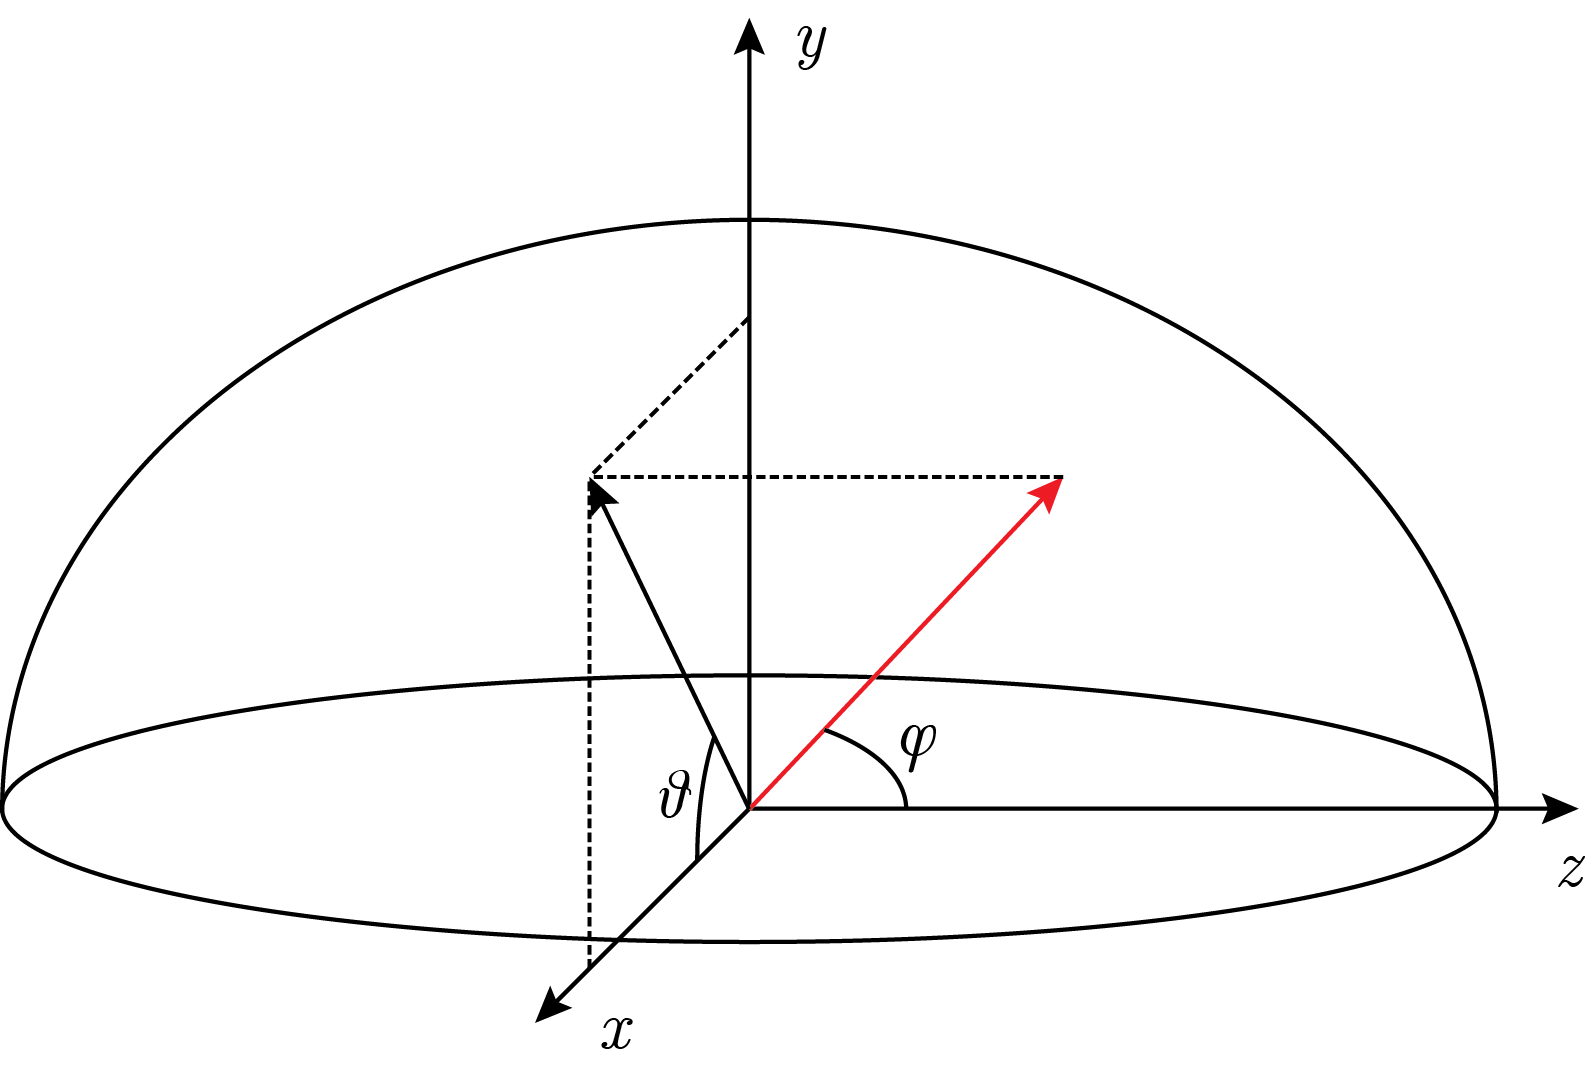
\includegraphics[width=.9\linewidth]{graphics/spherical.png}
\end{figure}

In Chapter~\ref{ch:method}, we briefly discussed that we construct the \emph{geometry buffer}
of a surface by using its UV-embedding. However, it is not obvious whether an arbitrary
UV-embedding can be applied for our model. Ideally, the model accepts any valid UV-embedding
and produces a corresponding albedo texture-map. However, there are several considerations
that make certain embeddings more useful than others. A good embedding should have the
following qualities:

\begin{itemize}
\renewcommand\labelitemi{--}
    \item Similarity of embeddings for similar surfaces is an important feature required for
        generalization capabilities of our model. I.e., if we feed in two similar car surfaces,
        we should expect similar UV-embeddings. This similarity allows the generator to
        learn to generate similar texture-maps for similar surfaces.
    \item General compactness of the embedding is also very important since we're restricted
        to using convolutions; any unassigned coordinates in the UV-embedding will take up space
        in the convolution input while not being used to produce the final texture-map.
    \item Conservation of surface connectivity in the UV-embedding ensures that operations that
        operate in local neighborhoods, such as convolutions, respect the surface connectivity.
        Otherwise, discontinuities caused by seams in the UV-embedding would create
        discontinuities along the seam when a generated texture-map is composited onto a surface.
    \item Low distortion is important due to the static size of the convolution filter used
        in the model. Applying a filter on a stretched out area of the embedding will
        shrink the effective size of the filter on the surface manifold and vice versa.
\end{itemize}

For our implementation, we normalize the UV-embeddings across all car surfaces using a
hemispherical parameterization. Given the $(x, y, z)$ coordinates of a point in the standard
Euclidean basis, we can compute its corresponding spherical coordinates $(r, \theta, \phi)$,
where the point is located a distance of $r$ away from the origin and oriented by the
azimuth angle $\theta$ and polar angle $\phi$. Using this change of coordinates, we construct
the hemispherical parameterization $(u, v) \in [0, 1]^2$ by discarding the radial distance $r$
and scaling $\theta$ and $\phi$ to a unit length. Since we're parameterizing a hemisphere,
(as opposed to a whole sphere) we scale $\theta$ by $\pi$ instead of $2 \pi$.

\begin{equation}
    (u, v) = (\theta / \pi, \phi / \pi)
\end{equation}

In general, the parameterization we described is not suitable for arbitrary shapes, especially
if the shape has overlapping points along a radial direction as these points will be assigned
to the same UV-coordinates. Fortunately, the roughly ellipsoid shape of car hulls allow us to
use this parameterization with minimal artifacts.

This parameterization is (1) similar between similar surfaces as long as the center
of each car model is standardized across models, (2) compact and roughly square since the
surface is roughly shaped like an ellipsoid, and (3) reflects the connectivity of the surface
well as our parameterization does not introduce any seams. Unfortunately, this parameterization
has high distortion near the poles of the parameterization. For the scope of this thesis we
do not address this issue, but we provide a discussion of a possible fix to this problem in
Section \ref{sec:distortion}.

\section{Dataset Generation}

We generate a synthetic dataset for model training using the ray tracer $\mathcal{R}_\Phi$
we described in Section \ref{sec:diffrtgan}, as well as a procedural surface weathering
texture-map generator $\mathcal{G}_0$~\cite{bhandari2018procedural}. In order to create a
diverse training dataset, we sample a random scene description $\Phi$ from a pool of car meshes,
base materials, environment maps, and camera parameters. We describe the distribution of assets
and their sampling strategies in more detail in Appendix \ref{app:system-overview}. Additionally,
we mark a subset of the materials as \emph{learnable} and composit the surface weathering
texture-map generated from $\mathcal{G}_0$ onto the base material of the surface using the
alpha-channel of the texture-map.

During training, each exemplar image from this dataset is loaded along with its corresponding
scene description $\Phi$ to aide in the training process. We evaluate our model $\mathcal{G}$
by comparing the fidelity of its results to $\mathcal{G}_0$. In Chapter~\ref{ch:experiment},
we discuss how the use of the scene description $\Phi$ of the training dataset affects the
performance of the model.

\section{Model Hyper-parameters}

\subsection{Network Architecture}

We adopt the network architecture choices by Zhou et al.'s model for non-stationary texture
synthesis~\cite{zhou2018non}. Our generator network is the
ResNet architecture by Johnson et al.~\cite{johnson2016perceptual}, featuring several
convolutions, followed by six residual blocks~\cite{he2016deep}, and several fractionally
strided convolutions. Our discriminator network is the PatchGAN architecture~\cite{isola2017image}.

\subsection{Loss Function}

Empirical results show that training with the Wasserstein GAN loss with gradient penalty as
proposed by Gulrajani et al.~\cite{gulrajani2017improved} produce the best results with the
fastest convergence rates, compared to the vanilla GAN loss~\cite{goodfellow2014generative}
and the LSGAN loss~\cite{mao2017least}. We present a comparison between these models in
Chapter~\ref{ch:experiment}.

\subsection{Training Process} \label{training-process}

The differentiable ray tracer~\cite{li2018differentiable} is a computation and memory
intensive operation, even when run on a GPU. Our experiments show that rendering an image
with resolution of $256 \times 256$, scene complexity of $\mathtt{\sim} 1,000,000$ vertices,
and Monte-Carlo sub-sampling rate of $200$ per pixel, takes $\mathtt{\sim} 0.3$ seconds in
the forward direction and $\mathtt{\sim} 9.0$ seconds in the backward direction (i.e.
computing the derivative); running multiple render operations in parallel on the GPU further
increases this runtime. We found that using a smaller Monte-Carlo sub-sampling rate in the
backward direction gives us a more reasonable runtime of $\mathtt{\sim}  0.9$ seconds at the cost
of accuracy of the computed derivatives.

Still, coupled with the large memory footprint the operation requires to store the scene
description and relevant metadata needed for derivative computations, training the model
with a large batch size is unfeasible unless we have a dedicated cluster of GPUs with
synchronized training. Due to these limitations, we conducted all experiments using batch size
of $1$ on a single GPU. \cite{zhu2017unpaired} shows that training GAN architectures with a batch
size of $1$ produces good results.
